\documentclass[10pt,a4paper]{article}
% Generated by build_short_report.py. Compile with pdflatex or on Overleaf.
\usepackage[T1]{fontenc}
\usepackage[utf8]{inputenc}
\usepackage{lmodern}
\usepackage{textcomp}
\usepackage[a4paper,margin=1.9cm,top=2.0cm,bottom=1.7cm]{geometry}
\usepackage{graphicx}
\usepackage{booktabs}
\usepackage{array}
\usepackage{float}
\usepackage{enumitem}
\usepackage{microtype}
\usepackage[font=footnotesize]{caption}
\usepackage{fancyhdr}
\usepackage{url}
\setlist[itemize]{leftmargin=1.2em,itemsep=1pt,topsep=2pt}
\setlength{\parindent}{0pt}
\setlength{\parskip}{3pt}
\pagestyle{fancy}\fancyhf{}
\lhead{\small RAI-FM (DSE428/DSE628), Assignment-4}\rhead{\small Payal Verma, 2611004}\cfoot{\small\thepage}
\renewcommand{\headrulewidth}{0.4pt}
\setlength{\headheight}{13pt}
\begin{document}
\thispagestyle{fancy}
\begin{center}
{\bfseries RAI-FM (DSE428/DSE628)}\\ {\bfseries Assignment-4}\\[4pt]
{\Large\bfseries Fairness Audit, Mitigation and Interpretability on Adult Income}\\[4pt]
Name: Payal Verma \qquad Roll No.: 2611004
\end{center}

\section*{Summary}

This report audits machine learning models on the Adult Income dataset for unfairness, makes one of them fairer, and uses interpretability methods to explain the result. All results are from 9,769 held-out test records, averaged over 3 seeds.

\begin{itemize}
  \item \textbf{Question 1: unfair for women.} A classifier on a deep autoencoder's code finds far fewer high-earning women than men (equal opportunity gap \textminus{}0.257). An SVM's gap is borderline (\textminus{}0.097 to \textminus{}0.108). Asian-Pacific Islander reconstruction error is 3.8 times White error.
  \item \textbf{Question 2: fixed on equal opportunity for women only.} Exponentiated Gradient moved the women's gap from \textminus{}0.257 to 0.029 at a cost of 0.006 accuracy. Demographic parity is still above 0.10 (\textminus{}0.115), and Black men did not benefit.
  \item \textbf{Question 3: relationship and marital-status drive the gap,} and relationship works as a proxy for sex. The fair loss moved the network's gap from \textminus{}0.090 to 0.022, but that network was already under the 0.10 cutoff for women overall, so it is an improvement rather than a clear change from unfair to fair.
\end{itemize}

\section*{1. Dataset}

Adult Income (Becker and Kohavi, 1996) has 48,842 records from the 1994 US census. The task is to predict whether a person earns more than \$50K (23.9\% do). Sex and race are audited, with Male and White as reference groups. The data was split 60/20/20, stratified on label, sex and race. Removing fnlwgt and education and one-hot encoding categories gives 84 input features without sex and race.

\begin{table}[H]
\centering\scriptsize
\setlength{\tabcolsep}{3pt}
\begin{tabular}{@{}>{\raggedright\arraybackslash}p{0.209\linewidth}>{\raggedright\arraybackslash}p{0.124\linewidth}>{\raggedright\arraybackslash}p{0.124\linewidth}>{\raggedright\arraybackslash}p{0.162\linewidth}@{}}
\toprule
\textbf{Group} & \textbf{Records} & \textbf{Share} & \textbf{Earning $>$\$50K} \\
\midrule
Male & 32,650 & 66.8\% & 30.4\% \\
Female & 16,192 & 33.2\% & 10.9\% \\
White & 41,762 & 85.5\% & 25.4\% \\
Black & 4,685 & 9.6\% & 12.1\% \\
Asian-Pac-Islander & 1,519 & 3.1\% & 26.9\% \\
Amer-Indian-Eskimo & 470 & 1.0\% & 11.7\% \\
Other & 406 & 0.8\% & 12.3\% \\
\bottomrule
\end{tabular}
\caption*{Table 1. Group sizes and income rates in the full dataset.}
\end{table}

\section*{2. Question 1: Fairness audit}

\noindent\fbox{\parbox{\dimexpr\linewidth-2\fboxsep-2\fboxrule}{\small \textbf{What was asked.} Implement at least two algorithms, at least one beyond logistic regression, PCA and K-means. Identify unfairness using task metrics (reconstruction error, accuracy) and fairness measures (demographic parity, equal opportunity).}}

\textbf{Models.} (1) A deep autoencoder (input-64-32-16-32-64-output) trained on reconstruction error, with a logistic regression on its frozen 16-dimensional code (``AE + LR'') so that fairness gaps can be measured, and PCA as a baseline. (2) An RBF SVM on a sample of 15,000 training records, with and without sex and race as inputs.

\textbf{Measures.} The demographic parity (DP) gap compares how often groups are predicted above \$50K. The equal opportunity (EO) gap compares true positive rates (TPR), meaning how often real high earners are recognised. A comparison counts as unfair if the EO gap is larger than 0.10 and its confidence interval excludes 0. Intervals use 2,000 bootstrap resamples: 95\% for sex and 98.75\% for race. Groups with fewer than 30 high earners are treated as inconclusive.

\begin{table}[H]
\centering\scriptsize
\setlength{\tabcolsep}{3pt}
\begin{tabular}{@{}>{\raggedright\arraybackslash}p{0.202\linewidth}>{\raggedright\arraybackslash}p{0.082\linewidth}>{\raggedright\arraybackslash}p{0.082\linewidth}>{\raggedright\arraybackslash}p{0.082\linewidth}>{\raggedright\arraybackslash}p{0.082\linewidth}>{\raggedright\arraybackslash}p{0.238\linewidth}>{\raggedright\arraybackslash}p{0.147\linewidth}@{}}
\toprule
\textbf{Model} & \textbf{Accuracy} & \textbf{Accuracy, women} & \textbf{TPR, women} & \textbf{TPR, men} & \textbf{EO gap (CI)} & \textbf{DP gap} \\
\midrule
SVM (no sex/race) & 0.858 & 0.934 & 0.524 & 0.621 & \textminus{}0.097 (\textminus{}0.154 to \textminus{}0.040) & \textminus{}0.183 \\
SVM (with sex/race) & 0.858 & 0.934 & 0.518 & 0.626 & \textbf{\textminus{}0.108} (\textminus{}0.165 to \textminus{}0.054) & \textminus{}0.186 \\
AE + LR & 0.839 & 0.919 & 0.344 & 0.601 & \textbf{\textminus{}0.257} (\textminus{}0.306 to \textminus{}0.209) & \textminus{}0.215 \\
\bottomrule
\end{tabular}
\caption*{Table 2. Test performance and gaps for women against men. Bold marks gaps that meet the verdict rule. Always predicting $\leq$\$50K scores 0.761 accuracy.}
\end{table}

\begin{figure}[H]
\centering
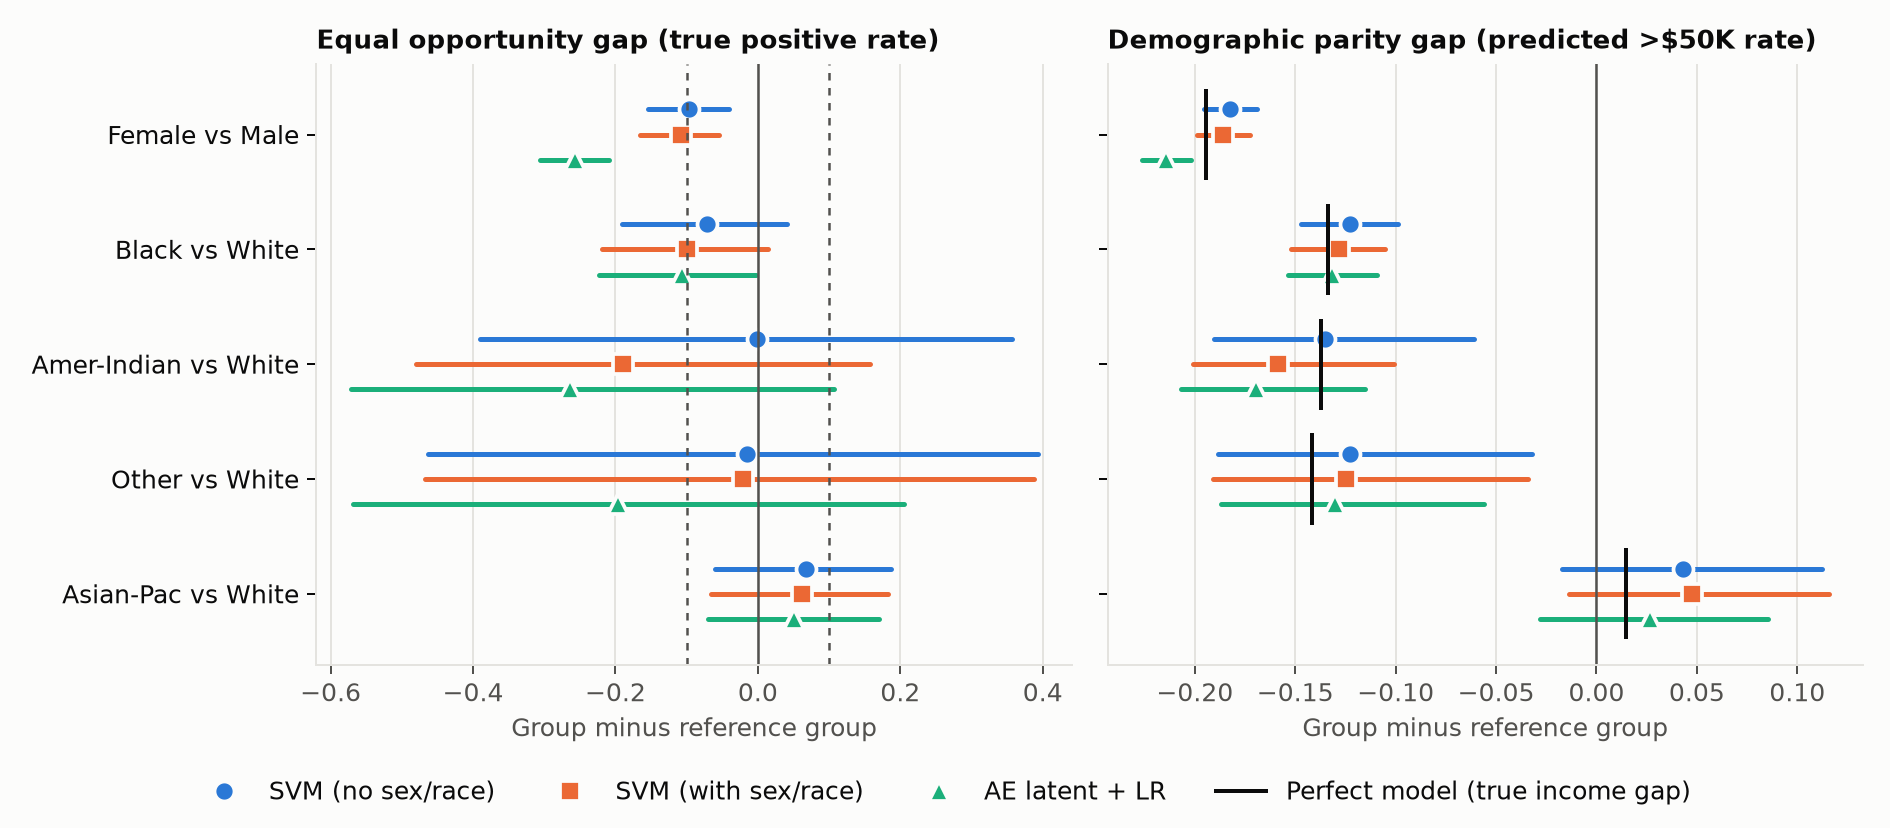
\includegraphics[width=0.90\linewidth]{results/fig2_fairness_gaps.png}
\caption*{Figure 1. Fairness gaps with confidence intervals. Dashed lines mark the $\pm$0.10 cutoff; black bars mark the true income gap.}
\end{figure}

\begin{itemize}
  \item \textbf{Accuracy hides the problem.} Women have higher accuracy but lower TPR than men in every model. Fewer women earn above \$50K, so predicting $\leq$\$50K is right more often for them, even while high-earning women are missed.
  \item \textbf{Race.} Only Black vs White under AE + LR meets the rule, and only just (\textminus{}0.107, interval \textminus{}0.224 to \textminus{}0.003). Amer-Indian-Eskimo and Other have 11 and 9 high earners, too few to judge.
  \item \textbf{Reconstruction error.} There is no meaningful gap by sex (0.0038 against 0.0036). Asian-Pac error is 3.8 times White (0.0125 against 0.0033) and Other 2.6 times. Native-country accounts for 73\% of Asian-Pac error, because rare countries are rebuilt poorly. The autoencoder's mean error is 0.0037 against 0.0096 for PCA.
\end{itemize}

\textbf{Verdict.} AE + LR is clearly unfair to women. The SVM is more accurate and borderline on the rule. Removing sex and race changed little (\textminus{}0.108 to \textminus{}0.097).

\section*{3. Question 2: Unfair to fair}

\noindent\fbox{\parbox{\dimexpr\linewidth-2\fboxsep-2\fboxrule}{\small \textbf{What was asked.} Make one algorithm fair, re-evaluate it with the same metrics, and identify the groups with the largest earlier disparities that are now reduced.}}

\textbf{Approach.} AE + LR was fixed because it had the clearest unfairness. Exponentiated Gradient (EG; Agarwal et al., 2018) was compared with reweighing (Kamiran and Calders, 2012), group thresholds (Hardt et al., 2016) and a group-balanced autoencoder. The method was chosen on validation data only: among methods that do not need a person's group at prediction and do not target demographic parity, keep those whose worst validation EO gap is at most 0.10, then take the highest validation accuracy. Only EG for equal opportunity by sex qualified.

\begin{table}[H]
\centering\scriptsize
\setlength{\tabcolsep}{3pt}
\begin{tabular}{@{}>{\raggedright\arraybackslash}p{0.307\linewidth}>{\raggedright\arraybackslash}p{0.108\linewidth}>{\raggedright\arraybackslash}p{0.081\linewidth}>{\raggedright\arraybackslash}p{0.081\linewidth}>{\raggedright\arraybackslash}p{0.081\linewidth}>{\raggedright\arraybackslash}p{0.081\linewidth}>{\raggedright\arraybackslash}p{0.081\linewidth}>{\raggedright\arraybackslash}p{0.081\linewidth}@{}}
\toprule
\textbf{Method} & \textbf{Worst EO gap, validation} & \textbf{Accuracy} & \textbf{Recall} & \textbf{TPR, women} & \textbf{TPR, men} & \textbf{EO gap, women} & \textbf{DP gap, women} \\
\midrule
Before (AE + LR) & 0.310 & 0.839 & 0.562 & 0.344 & 0.601 & \textminus{}0.257 & \textminus{}0.215 \\
\textbf{EG equal opportunity, sex (chosen)} & \textbf{0.013} & \textbf{0.833} & \textbf{0.511} & \textbf{0.535} & \textbf{0.506} & \textbf{0.029} & \textbf{\textminus{}0.115} \\
EG equal opportunity, sex $\times$ race & 0.121 & 0.788 & 0.318 & 0.349 & 0.313 & 0.037 & \textminus{}0.078 \\
EG demographic parity, sex & 0.138 & 0.809 & 0.393 & 0.541 & 0.367 & 0.175 & \textminus{}0.016 \\
Reweighing & 0.126 & 0.841 & 0.538 & 0.465 & 0.551 & \textminus{}0.085 & \textminus{}0.158 \\
Group thresholds, sex $\times$ race & 0.156 & 0.835 & 0.556 & 0.540 & 0.559 & \textminus{}0.019 & \textminus{}0.141 \\
Balanced AE (sqrt weights) + LR & 0.248 & 0.839 & 0.563 & 0.395 & 0.593 & \textminus{}0.198 & \textminus{}0.202 \\
Balanced AE (full weights) + LR & 0.305 & 0.838 & 0.554 & 0.333 & 0.594 & \textminus{}0.260 & \textminus{}0.211 \\
\bottomrule
\end{tabular}
\caption*{Table 3. Methods tried. Columns after the second use the test set.}
\end{table}

\begin{table}[H]
\centering\scriptsize
\setlength{\tabcolsep}{3pt}
\begin{tabular}{@{}>{\raggedright\arraybackslash}p{0.176\linewidth}>{\raggedright\arraybackslash}p{0.065\linewidth}>{\raggedright\arraybackslash}p{0.195\linewidth}>{\raggedright\arraybackslash}p{0.195\linewidth}>{\raggedright\arraybackslash}p{0.176\linewidth}>{\raggedright\arraybackslash}p{0.121\linewidth}@{}}
\toprule
\textbf{Comparison} & \textbf{High earners} & \textbf{EO gap before (CI)} & \textbf{EO gap after (CI)} & \textbf{Reduction (CI)} & \textbf{Result} \\
\midrule
Women vs men & 354 & \textbf{\textminus{}0.257} (\textminus{}0.306 to \textminus{}0.209) & 0.029 (\textminus{}0.022 to 0.080) & 0.228 (0.131 to 0.293) & Reduced \\
White women vs White men & 309 & \textbf{\textminus{}0.265} (\textminus{}0.337 to \textminus{}0.196) & 0.019 (\textminus{}0.060 to 0.096) & 0.246 (0.109 to 0.314) & Reduced \\
Black vs White & 113 & \textbf{\textminus{}0.107} (\textminus{}0.224 to \textminus{}0.003) & \textminus{}0.085 (\textminus{}0.201 to 0.023) & 0.022 (\textminus{}0.041 to 0.088) & Not shown \\
Black men vs White men & 87 & \textminus{}0.127 (\textminus{}0.287 to 0.013) & \textbf{\textminus{}0.133} (\textminus{}0.266 to \textminus{}0.004) & \textminus{}0.007 (\textminus{}0.087 to 0.061) & No change \\
\bottomrule
\end{tabular}
\caption*{Table 4. Before and after EG, with paired bootstrap intervals. Bold marks gaps that meet the verdict rule.}
\end{table}

\begin{figure}[H]
\centering
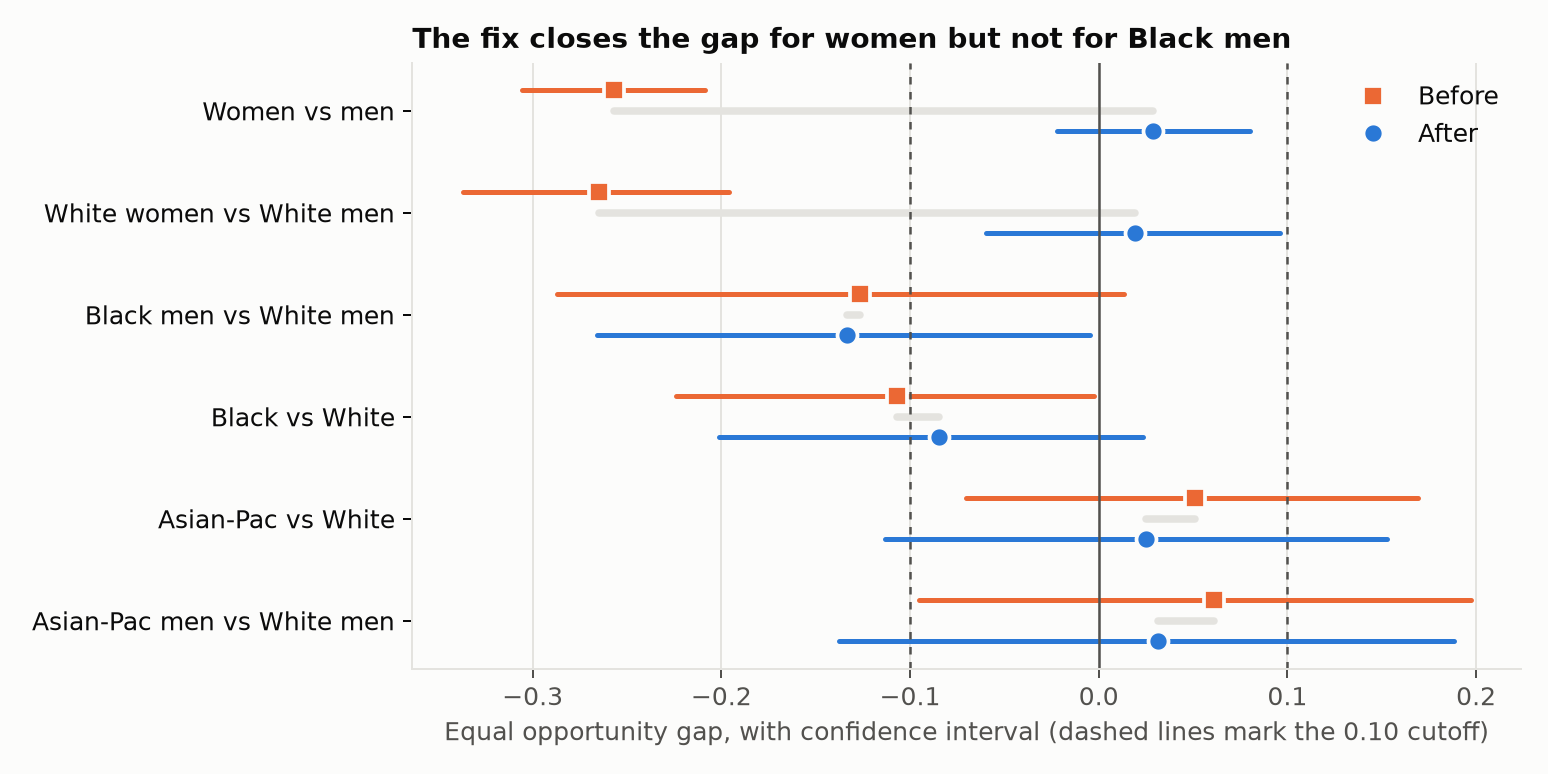
\includegraphics[width=0.62\linewidth]{results/q2/fig1_before_after_gaps.png}
\caption*{Figure 2. Equal opportunity gaps before and after EG, with confidence intervals.}
\end{figure}

\begin{itemize}
  \item \textbf{Groups improved.} Women and White women had the largest measurable disparities, and both are now reduced. Part of this came from lowering men's rate: TPR rose from 0.344 to 0.535 for women and fell from 0.601 to 0.506 for men.
  \item \textbf{Not fixed.} The women's DP gap went from \textminus{}0.215 to \textminus{}0.115, still above 0.10. Black men's gap did not detectably change, and their TPR fell from 0.479 to 0.379. EG decisions are randomised, so the same person can get different answers.
  \item \textbf{Reconstruction.} Balanced training narrowed the Asian-Pac to White ratio from 3.96 to 3.03 (averaged across seeds), but the change is about the size of the seed variation and partly comes from raising White error, so it is not established as a fix.
  \item \textbf{Trade-off.} EG for demographic parity nearly closes that gap (\textminus{}0.016) but overshoots on equal opportunity (0.175), with accuracy at 0.809. Because income rates differ by sex, the two measures generally cannot both be satisfied.
\end{itemize}

\textbf{Verdict.} The model is now fair for women on equal opportunity under this rule, at a small accuracy cost (0.839 to 0.833). It is not fair in every sense.

\section*{4. Question 3: Interpretability of unfairness and fairness}

\noindent\fbox{\parbox{\dimexpr\linewidth-2\fboxsep-2\fboxrule}{\small \textbf{What was asked.} Use at least two interpretability techniques to investigate whether features contribute disproportionately to particular groups or make the network unfair, and whether it became fair after the fair optimization loss.}}

\textbf{Fair loss.} EG is not a loss, so a network was also fine-tuned on binary cross-entropy + $\lambda$(TPR\textsubscript{women} \textminus{} TPR\textsubscript{men})$^2$, using soft TPR. $\lambda$ = 0 gives the ``before'' network, and $\lambda$ = 2 was chosen on validation data. No model sees sex or race at prediction.

\textbf{Techniques.} \textbf{SHAP} (Lundberg and Lee, 2017): exact Shapley values on the log-odds over all 2\textsuperscript{10} combinations of the 10 original features. \textbf{Vanilla gradients} (Simonyan et al., 2014): gradient size and signed contribution. A \textbf{scramble test} also shuffles each feature across test records without retraining and re-measures the EO gap, because attributions describe scores while fairness depends on decisions.

\begin{table}[H]
\centering\scriptsize
\setlength{\tabcolsep}{3pt}
\begin{tabular}{@{}>{\raggedright\arraybackslash}p{0.253\linewidth}>{\raggedright\arraybackslash}p{0.081\linewidth}>{\raggedright\arraybackslash}p{0.072\linewidth}>{\raggedright\arraybackslash}p{0.090\linewidth}>{\raggedright\arraybackslash}p{0.118\linewidth}>{\raggedright\arraybackslash}p{0.090\linewidth}>{\raggedright\arraybackslash}p{0.108\linewidth}>{\raggedright\arraybackslash}p{0.090\linewidth}@{}}
\toprule
\textbf{Model} & \textbf{Accuracy} & \textbf{Recall} & \textbf{Women vs men} & \textbf{White women vs White men} & \textbf{Black vs White} & \textbf{Black men vs White men} & \textbf{DP gap, women} \\
\midrule
AE + LR (before) & 0.839 & 0.562 & \textbf{\textminus{}0.257} & \textbf{\textminus{}0.265} & \textbf{\textminus{}0.107} & \textminus{}0.127 & \textminus{}0.215 \\
AE + EG (after) & 0.833 & 0.511 & 0.029 & 0.019 & \textminus{}0.092 & \textbf{\textminus{}0.142} & \textminus{}0.116 \\
Network, no fair loss (before) & 0.849 & 0.616 & \textminus{}0.090 & \textbf{\textminus{}0.110} & \textminus{}0.063 & \textminus{}0.101 & \textminus{}0.190 \\
Network, fair loss (after) & 0.847 & 0.597 & 0.022 & 0.008 & \textminus{}0.070 & \textminus{}0.107 & \textminus{}0.150 \\
\bottomrule
\end{tabular}
\caption*{Table 5. Performance and EO gaps for the four models. Bold marks gaps that meet the verdict rule. EG gaps here use the expected value of its random decision.}
\end{table}

\textbf{Did the network become fair?} Partly. The women's gap moved from \textminus{}0.090 to 0.022, and White women no longer meet the rule (\textminus{}0.110 to 0.008). But the network was already under the cutoff for women overall, neither reduction is statistically established (intervals \textminus{}0.036 to 0.124 and \textminus{}0.050 to 0.153), the DP gap stays large (\textminus{}0.150), and Black men did not improve. Fine-tuning the encoder for income at all moved the gap more (\textminus{}0.257 to \textminus{}0.090) than the fair loss did.

\begin{figure}[H]
\centering
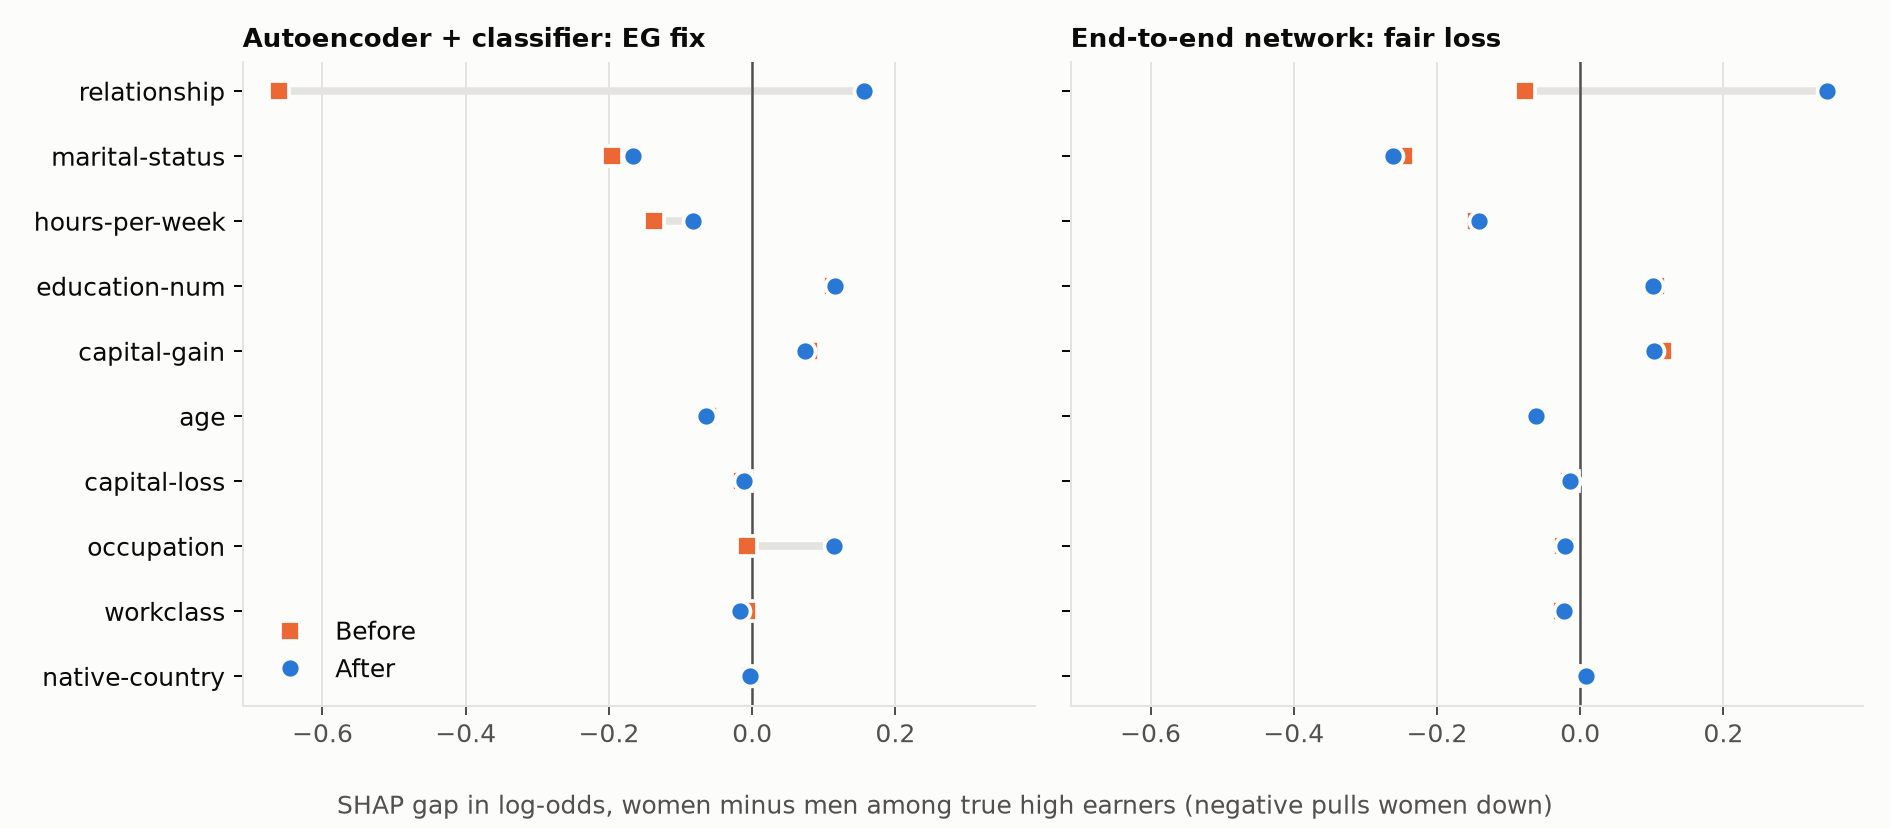
\includegraphics[width=0.76\linewidth]{results/q3/fig1_shap_gap_women_men.png}
\caption*{Figure 3. SHAP gaps between women and men among high earners, before and after each fix.}
\end{figure}

\begin{table}[H]
\centering\scriptsize
\setlength{\tabcolsep}{3pt}
\begin{tabular}{@{}>{\raggedright\arraybackslash}p{0.183\linewidth}>{\raggedright\arraybackslash}p{0.119\linewidth}>{\raggedright\arraybackslash}p{0.119\linewidth}>{\raggedright\arraybackslash}p{0.110\linewidth}>{\raggedright\arraybackslash}p{0.110\linewidth}>{\raggedright\arraybackslash}p{0.137\linewidth}>{\raggedright\arraybackslash}p{0.137\linewidth}@{}}
\toprule
\textbf{Category} & \textbf{Share of high-earning women} & \textbf{Share of high-earning men} & \textbf{AE + LR (before)} & \textbf{AE + EG (after)} & \textbf{Network, no fair loss} & \textbf{Network, fair loss} \\
\midrule
Husband & 0.0\% & 88.6\% & +1.18 & +0.80 & +0.94 & +0.77 \\
Wife & 63.6\% & 0.0\% & +0.75 & +1.36 & +1.31 & +1.71 \\
Unmarried & 8.5\% & 1.4\% & \textminus{}0.28 & +0.35 & \textminus{}0.56 & \textminus{}0.51 \\
\bottomrule
\end{tabular}
\caption*{Table 6. Mean SHAP value of relationship by category, among high earners. Husband and Wife are held by one sex only.}
\end{table}

\begin{table}[H]
\centering\scriptsize
\setlength{\tabcolsep}{3pt}
\begin{tabular}{@{}>{\raggedright\arraybackslash}p{0.204\linewidth}>{\raggedright\arraybackslash}p{0.278\linewidth}>{\raggedright\arraybackslash}p{0.111\linewidth}>{\raggedright\arraybackslash}p{0.111\linewidth}>{\raggedright\arraybackslash}p{0.111\linewidth}>{\raggedright\arraybackslash}p{0.111\linewidth}@{}}
\toprule
\textbf{Comparison} & \textbf{Feature scrambled} & \textbf{AE + LR (before)} & \textbf{AE + EG (after)} & \textbf{Network, no fair loss} & \textbf{Network, fair loss} \\
\midrule
Women vs men & (nothing scrambled) & \textminus{}0.257 & 0.029 & \textminus{}0.090 & 0.022 \\
Women vs men & relationship & \textminus{}0.059 & \textminus{}0.015 & \textminus{}0.081 & \textminus{}0.081 \\
Women vs men & relationship + marital-status & \textminus{}0.010 & 0.028 & \textminus{}0.010 & \textminus{}0.010 \\
Black men vs White men & (nothing scrambled) & \textminus{}0.127 & \textminus{}0.142 & \textminus{}0.101 & \textminus{}0.107 \\
Black men vs White men & education-num & \textminus{}0.063 & \textminus{}0.060 & \textminus{}0.055 & \textminus{}0.051 \\
\bottomrule
\end{tabular}
\caption*{Table 7. EO gap after scrambling, without retraining. Mean over 3 seeds and 5 shuffles. No intervals were computed.}
\end{table}

\begin{figure}[H]
\centering
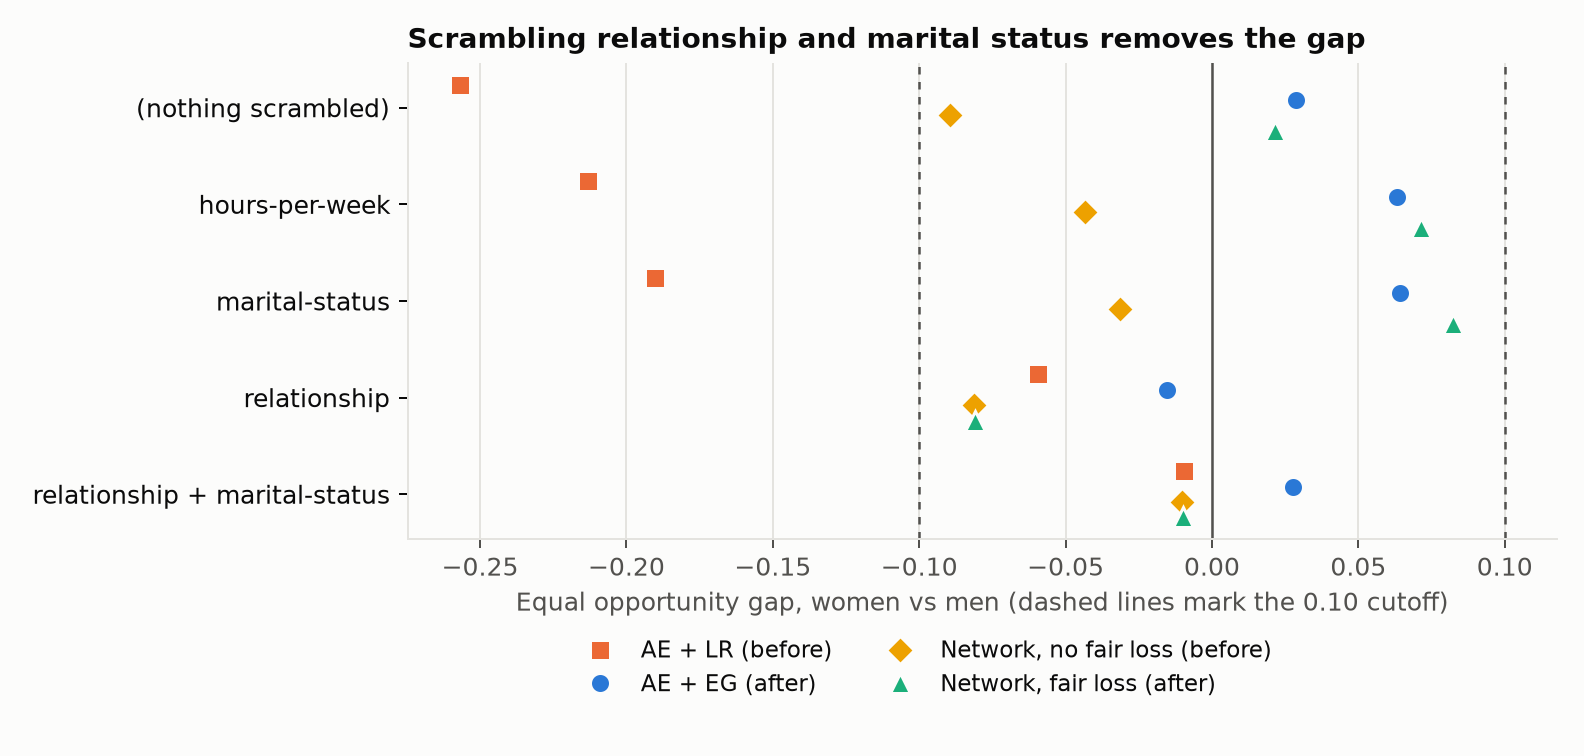
\includegraphics[width=0.62\linewidth]{results/q3/fig2_scramble_test.png}
\caption*{Figure 4. Women vs men equal opportunity gap after scrambling each feature. Only the features that move the gap most are shown.}
\end{figure}

\begin{itemize}
  \item \textbf{Which features.} Relationship is the largest SHAP gap in AE + LR (\textminus{}0.661) and marital-status in the network (\textminus{}0.246). Scrambling both nearly removes the women's gap (\textminus{}0.257 to \textminus{}0.010).
  \item \textbf{Relationship is a proxy for sex.} 89\% of high-earning men are Husbands and 64\% of high-earning women are Wives, and these category mixes reproduce the full SHAP gap (\textminus{}0.663 against \textminus{}0.661). Women and men in the same shared category get almost the same value.
  \item \textbf{The bias is offset, not removed.} After the fair loss, Wife scores further above Husband (+1.71 against +0.77), and scrambling relationship brings the gap back to \textminus{}0.081. The marital-status gap stays (\textminus{}0.262). Unmarried stays at \textminus{}0.51, so parity rests largely on wives.
  \item \textbf{Black men have an additional driver.} Education-num has their largest SHAP gap (\textminus{}0.224), and EG leaves it unchanged (\textminus{}0.226). A fix aimed at sex would not be expected to change it.
  \item \textbf{Do the techniques agree?} Signed gradient contributions agree with SHAP (correlation 0.987 to 0.999), though they are not fully independent evidence. Gradient size does not: it ranks native-country highest, while scrambling native-country leaves the gap almost unchanged (\textminus{}0.257 to \textminus{}0.256).
\end{itemize}

\begin{table}[H]
\centering\scriptsize
\setlength{\tabcolsep}{3pt}
\begin{tabular}{@{}>{\raggedright\arraybackslash}p{0.351\linewidth}>{\raggedright\arraybackslash}p{0.625\linewidth}@{}}
\toprule
\textbf{Question} & \textbf{Answer} \\
\midrule
Do some features contribute disproportionately for particular groups? & \textbf{Yes.} Relationship and marital-status for women; education-num as well as these two for Black men. \\
Do those features make the model unfair? & \textbf{Yes, for these trained models.} Scrambling the first two nearly removes the women's gap. \\
Why do they do this? & Relationship works as a proxy for sex, because Husband and Wife are sex-specific categories. Marital-status is a weaker signal. \\
Did the network become fair after the fair loss? & \textbf{Partly.} Gaps are near zero and White women no longer meet the rule, but the network was under the cutoff for women overall, the reductions are not statistically established, and demographic parity is still above 0.10. \\
Did the model's reliance on these features end? & \textbf{No.} The fixes push the proxy in women's favour, offsetting the bias rather than removing it. \\
\bottomrule
\end{tabular}
\caption*{Table 8. Answers to Question 3.}
\end{table}

\section*{5. Limitations}

The data is from 1994, and sex and race are recorded in broad categories. Small groups give wide intervals, so ``no gap found'' does not mean ``fair''. Several verdicts sit close to the 0.10 cutoff. Intervals reflect test-set sampling, not differences between training runs, and 3 seeds estimate seed variation only roughly. SHAP and scrambling show what these trained models rely on, not what causes income. The scramble test has no intervals and did not record accuracy, so it supports SHAP rather than proving it. LIME, attention and prototypes were not tried, and neither model is a foundation model.

\section*{6. Conclusion}

Fairness problems were found, and they depend on the model and the metric. Accuracy alone would have pointed in the wrong direction, and removing sensitive columns did little. EG closed the equal opportunity gap for women at a small accuracy cost, and the fair loss brought the network's gap close to zero, but neither is fairness in every sense. Interpretability explains why: relationship stands in for sex, and the fair models shift it in women's favour rather than stop using it. Parity on a chosen measure can be reached without removing the underlying dependence, so an audit should look inside the model as well as at its gaps.

{\small \textbf{References.} Agarwal et al. (2018), A Reductions Approach to Fair Classification, ICML. Becker and Kohavi (1996), Adult, UCI Machine Learning Repository. Hardt, Price and Srebro (2016), Equality of Opportunity in Supervised Learning, NeurIPS. Kamiran and Calders (2012), Data Preprocessing Techniques for Classification without Discrimination, Knowledge and Information Systems. Lundberg and Lee (2017), A Unified Approach to Interpreting Model Predictions, NeurIPS. Simonyan, Vedaldi and Zisserman (2014), Deep Inside Convolutional Networks, ICLR Workshop.}

{\small \textbf{Code.} \url{https://github.com/payalv623/fairness-audit-and-interpretability}}

\end{document}
